% -----------------------------------------------------------------------------
\index{OpenQuake-engine!hazard} 
The hazard component of the OpenQuake-engine builds on top of the 
\gls{acr:hazlib}, a python-based library containing
tools for PSHA calculation. 
%
The web repository of this library is available at the following address: 
\href{http://gitub.com/gem/oq-hazardlib}{http://gitub.com/gem/oq-hazardlib}.
%
In this section we briefly illustrate the main properties of the 
hazard component of the engine. 
%
In particular, we will describe the main typologies of sources supported 
and the main calculation workflows available.
%
\section{Source typologies}
\index{Source type}
A general \gls{acr:oqe} Seismic Source model contains a list
of sources belonging to a finite set of possible typologies. 
Each source type is defined by a set of parameters - called 
source data - essential for specifying source geometry and 
seismicity occurrence characteristics.
%
Currently the OpenQuake-engine supports the following source types: 
\begin{itemize}
	\item Sources for modelling distributed seismicity:
	\begin{itemize}
		\item \Gls{pointsource} - The elemental source type use to model 
			distributed seismicity. Grid and area sources described below
			are basically two different containers of point sources.
		\item \Gls{areasource} - So far, the most frequently adopted source 
    		type in national and regional PSHA models.
		\item Grid sources - Can be considered a replacement 
    		for area sources since they both model distributed seismicity.
	\end{itemize}
	\item Fault sources with floating ruptures:
	\begin{itemize}
		\item \Gls{simplefaultsource} - The simplest fault model in OpenQuake. 
    		This typology is habitually used to describe shallow seismogenic 
    		faults.
		\item \Gls{complexfaultsource} - Often used to model subduction interface 
			sources with a complex geometry. 
	\end{itemize}
	\item Fault sources with ruptures always covering the entire fault surface:
	\begin{itemize}
		\item \Gls{charfaultsource} - A typology of source where ruptures
		always fill the entire fault surface.
	\end{itemize}
\end{itemize}
Moreover, there are some basic assumptions accepted in the definition of these 
source typologies such as:
\begin{itemize}
	\item In the case of area and fault sources, the seismicity is homogeneously 
		distributed over the source; 	
	\item Seismicity temporal occurrence follows a Poissonian model; 
\end{itemize}
% . . . . . . . . . . . . . . . . . . . . . . . . . . . . . . . . . . . . . . .
\subsection{Source typologies for modelling distributed seismicity}
\subsubsection{Point sources}
\label{hazard:seismic_source_types:pointSources}
\index{Source type!point}
\index{Point source|see{Source type}}
% ..............................................................................
% . . . . . . . . . . . . . . . . . . . . . . . . . . . . . . . . . . . > Figure
\begin{figure}[!ht]
\centering
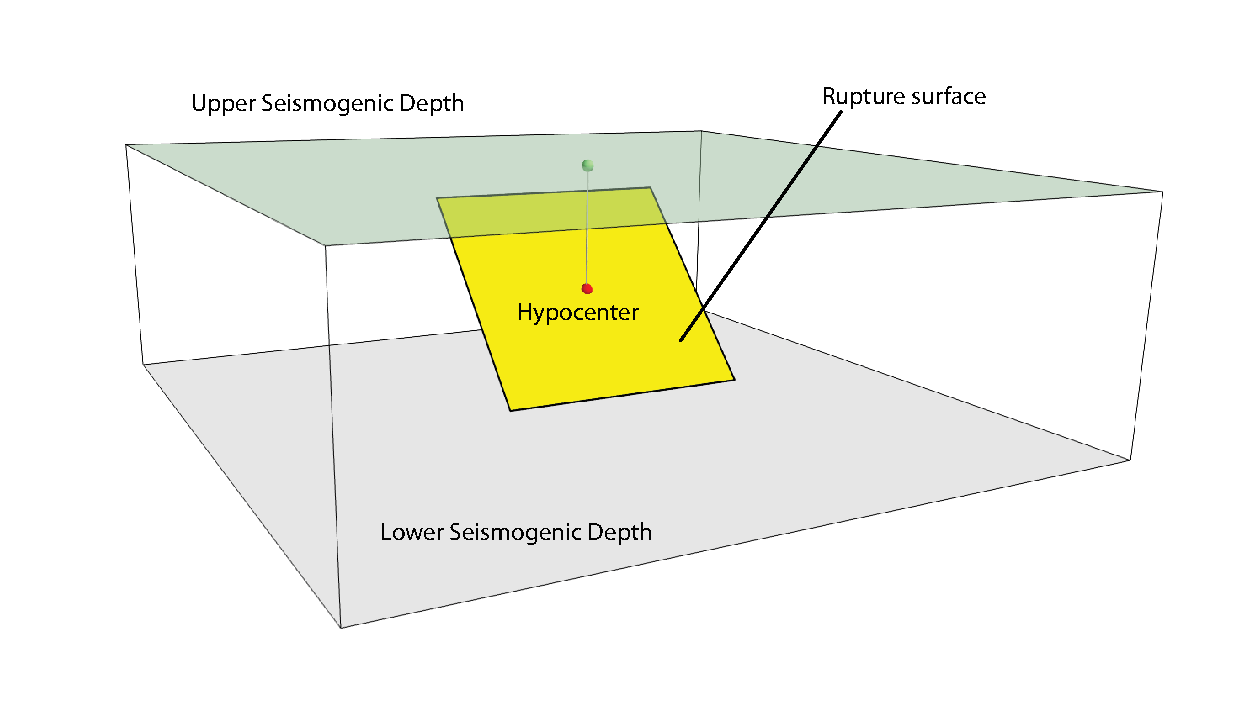
\includegraphics[width=10cm]{./figures/hazard/single_rupture.eps}
\caption{Single rupture}
\label{fig:single_rupture}
\end{figure}
% . . . . . . . . . . . . . . . . . . . . . . . . . . . . . . . . . . . < Figure
% ..............................................................................
Point source is the elemental source type adopted in the OpenQuake engine 
to model distributed seismicity. These are the basic assumptions used to 
generate finite ruptures with point sources:
\begin{itemize}
	\item ruptures have a rectangular shape
	\item rupture's hypocenter is located in the middle of the rupture
	\item ruptures are limited at the top and at the bottom by two planes 
	parallel to the topographic surface and placed at two characteristic 
	depths named upper and lower seismogenic depths, respectively.
\end{itemize} 
%
%  . . . . . . . . . . . . . . . . . . . . . . . . . . . . . . . . . . . . . . . 
\paragraph{Source data}
%
For each point source (i.e. grid node) the following parameters are requested
(Figure \ref{fig:single_rupture} shows some of the parameters described below, 
together with an example of rupture):
\begin{itemize}
\item The coordinates of the point (i.e. Longitude and Latitude in decimal 
    degrees)
\item The upper and lower seismogenic depths;
\item One \gls{mfd};
\item One magnitude-scaling relationship;
\item The rupture aspect ratio;
\item A distribution of nodal planes i.e. one (or several) instances 
    of the following set of parameters:
\begin{itemize}
    \item \gls{strike}
    \item \gls{dip}
    \item \gls{rake}
\end{itemize}
\item A magnitude independent depth distribution of hypocenters. 
\end{itemize}
%
Figure \ref{fig:point_source_multiple_ruptures} shows multiple ruptures 
of different magnitude centered on the single hypocentre allowed 
by this point source. Ruptures are created by conserving the area obtained
from magnitude through a magnitude-area scaling relatioship.
% ..............................................................................
% . . . . . . . . . . . . . . . . . . . . . . . . . . . . . . . . . . . > Figure
\begin{figure}[ht!]
\centering
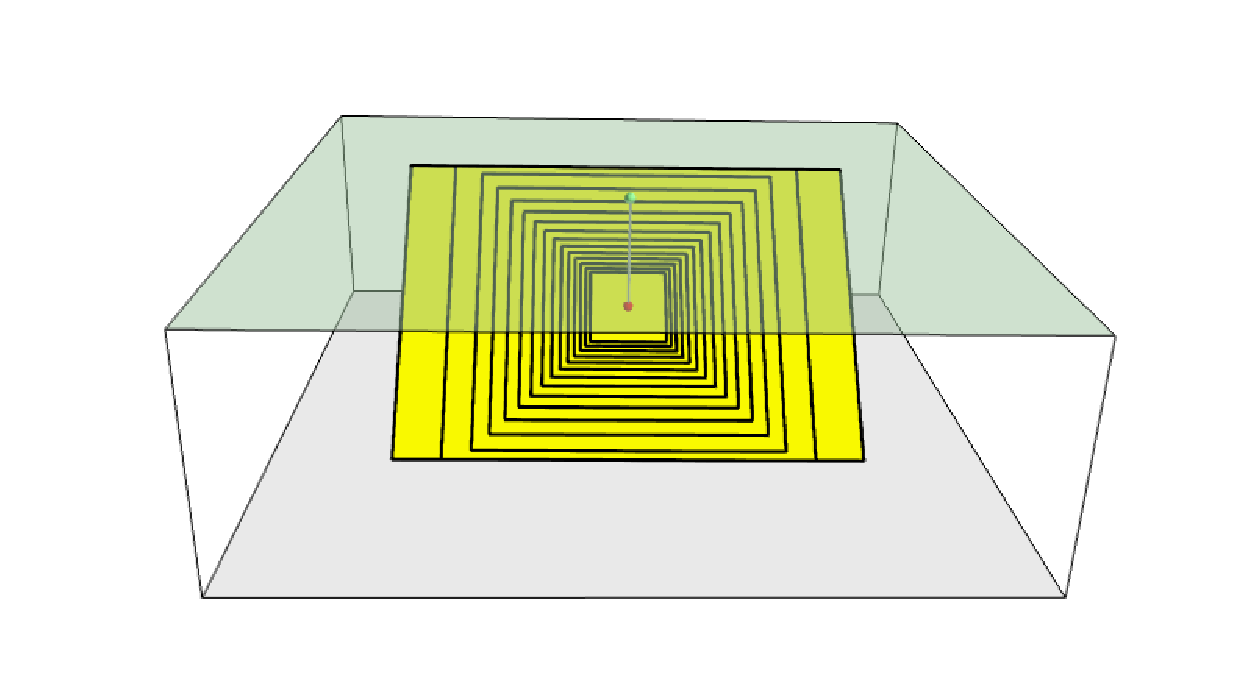
\includegraphics[width=10cm]{./figures/hazard/point_source_multiple_ruptures.ps}
\caption{Point source with multiple ruptures. Note the change in the aspect 
ratio once the rupture width fills the entire seismogenic layer.}
\label{fig:point_source_multiple_ruptures}
\end{figure}
% . . . . . . . . . . . . . . . . . . . . . . . . . . . . . . . . . . . < Figure
% ..............................................................................
Below we provide the excerpt of an .xml file used to describe the 
properties of a point source of a seismic source model.
\label{page:xml_point}
\begin{Verbatim}[frame=single, commandchars=\\\{\}, fontsize=\footnotesize,
    numbers=left, numbersep=2pt]
<pointSource id="1" name="point" tectonicRegion="Stable Continental Crust">
    <pointGeometry>
        <gml:Point>
            <gml:pos>-122.0 38.0</gml:pos>
        </gml:Point>
        <upperSeismoDepth>0.0</upperSeismoDepth>
        <lowerSeismoDepth>10.0</lowerSeismoDepth>
    </pointGeometry>
    <magScaleRel>WC1994</magScaleRel>
    <ruptAspectRatio>0.5</ruptAspectRatio>
    <truncGutenbergRichterMFD aValue="-3.5" bValue="1.0" minMag="5.0" 
			maxMag="6.5" />
    <nodalPlaneDist>
        <nodalPlane probability="0.3" strike="0.0" dip="90.0" rake="0.0" />
        <nodalPlane probability="0.7" strike="90.0" dip="45.0" rake="90.0" />
    </nodalPlaneDist>
    <hypoDepthDist>
        <hypoDepth probability="0.5" depth="4.0" />
        <hypoDepth probability="0.5" depth="8.0" />
    </hypoDepthDist>
</pointSource>
\end{Verbatim}
In this example, ruptures occur on two possible nodal planes and two 
hypocentral depths. Figure \ref{fig:point_source_ruptures} shows all 
the possible ruptures generated by the point source specified above.

% ..............................................................................
% . . . . . . . . . . . . . . . . . . . . . . . . . . . . . . . . . . . > Figure
\begin{figure}[!ht]
\centering
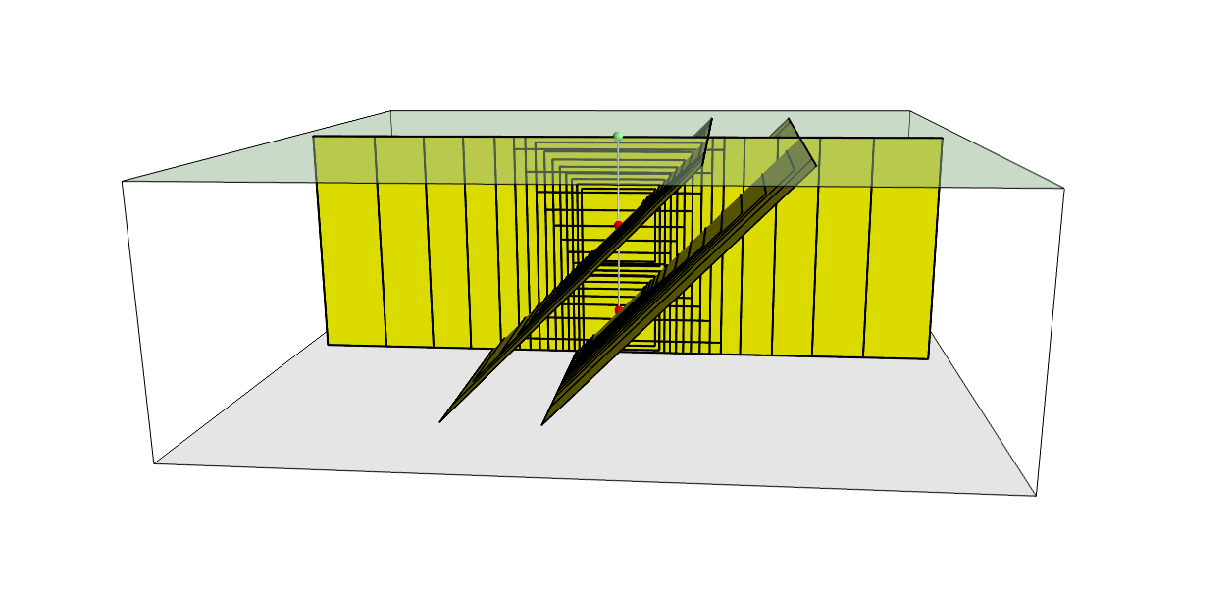
\includegraphics[width=10cm]{./figures/hazard/pointsrc_2strike_2hypodep.ps}
\caption{Ruptures produced by the source created using the information 
    in the example .xml file described at page \pageref{page:xml_point}.}
\label{fig:point_source_ruptures}
\end{figure}
% . . . . . . . . . . . . . . . . . . . . . . . . . . . . . . . . . . . < Figure
% ..............................................................................
%
% . . . . . . . . . . . . . . . . . . . . . . . . . . . . . . . . . . . . . . .
\subsubsection{Grid sources}
\label{hazard:seismic_source_types:gridSources}
\index{Source type!grid}
\index{Grid source|see{Source type}}
% 
A grid source is simply a collection of
point sources distributed over a regular grid (usually equally spaced in 
longitude and latitude).
%
In \gls{psha} a grid source can be considered a model alternative to area 
sources, since they both model distributed seismicity. 
%
Indeed, grid source is a typology used to reproduce a distributed 
seismicity process - usually involving events of low and intermediate 
magnitudes. 

Grid sources usually are computed using seismicity smoothing algorithms 
\citep[][amongst many others]{frankel1995,woo1996}. 
%
The use of this source type brings some advantages compared to area sources, 
since (1) it removes most of the unavoidable degree of subjectivity due to 
the definition of the geometries of the area sources and (2) it produces
a spatial pattern of seismicity that is usually closer to what observed in 
the reality. 
Nevertheless, some smoothing algorithms require an a-priori definition of 
some setup parameters that expose the calculation to a certain degree of 
partiality.

Grid sources are modelled in \gls{acr:oqe} simply as a set of point sources. 
%  . . . . . . . . . . . . . . . . . . . . . . . . . . . . . . . . . . . . . . . 
\subsubsection{Area sources}
\label{hazard:seismic_source_types:areaSources}
\index{Source type!area} 
\index{Area source|see{Source type}}
%
Area sources describe the seismicity occurring over wide areas where  
identification and characterization - i.e. the unambiguous definition 
of position, geometry and seismicity occurrence parameters - of single 
fault structures is difficult. 

From a computation standpoint area sources are comparable to grid sources.
The \gls{acr:oqe} using the source data parameters (see below)  
creates an equally spaced in distance grid of point sources where
each point has the same seismicity occurrence properties (i.e. rate
of events generated).

Below we provide a brief description of the parameters necessary to 
completely describe an area source:
%
%  . . . . . . . . . . . . . . . . . . . . . . . . . . . . . . . . . . . . . . . 
\paragraph{Source data}
\begin{itemize}
\item A polygon defining the external border of the area. 
The current version of OQ doesn't support the definition 
of internal borders
\item The upper and lower seismogenic depths;
\item One \gls{mfd};
\item One magnitude-scaling relationship;
\item The rupture aspect ratio;
\item A distribution of nodal planes i.e. one (or several) instances 
    of the following set of parameters:
\begin{itemize}
	\item strike
	\item dip
	\item rake
\end{itemize}
\item A magnitude independent depth distribution of hypocenters. 
\end{itemize}

Below we provide the exerpt of an .xml file used to describe the properties of
an area source of a seismic source model.
\begin{Verbatim}[frame=single, commandchars=\\\{\}, fontsize=\footnotesize,
numbers=left, numbersep=2pt]
<areaSource id="1" name="Quito" tectonicRegion="Active Shallow Crust">
    <areaGeometry>
        <gml:Polygon>
            <gml:exterior>
                <gml:LinearRing>
                    <gml:posList>
                     -122.5 37.5
                     -121.5 37.5
                     -121.5 38.5
                     -122.5 38.5
                    </gml:posList>
                </gml:LinearRing>
            </gml:exterior>
        </gml:Polygon>
        <upperSeismoDepth>0.0</upperSeismoDepth>
        <lowerSeismoDepth>10.0</lowerSeismoDepth>
    </areaGeometry>
    <magScaleRel>PeerMSR</magScaleRel>
    <ruptAspectRatio>1.5</ruptAspectRatio>
    <incrementalMFD minMag="6.55" binWidth="0.1">
        <occurRates>0.0010614989 8.8291627E-4 7.3437777E-4 6.108288E-4 
				5.080653E-4</occurRates>
    </incrementalMFD>
    <nodalPlaneDist>
        <nodalPlane probability="0.3" strike="0.0" dip="90.0" rake="0.0"/>
        <nodalPlane probability="0.7" strike="90.0" dip="45.0" rake="90.0"/>
    </nodalPlaneDist>
    <hypoDepthDist>
        <hypoDepth probability="0.5" depth="4.0" />
        <hypoDepth probability="0.5" depth="8.0" />
    </hypoDepthDist>
</areaSource>
\end{Verbatim}
The ruptures generated inside this area source follow to possible nodal 
planes and have hypocenters at two depths. 
%
%  . . . . . . . . . . . . . . . . . . . . . . . . . . . . . . . . . . . . . . .
\subsection{Fault source with floating ruptures}
%
Fault sources are classified according to the method adopted to 
distribute ruptures over the fault surface. Two are the option currently 
supported: 
\begin{itemize}
    \item Ruptures with a surface lower than the whole fault surface are 
        floated so as to cover as much as possible homogeneously the fault
        surface.
        This model is compatible with almost all the possible 
        magnitude-frequency distributions.
    \item Ruptures always fill the entire fault surface. This model is 
        compatible only with characteristic models (\`{a} la 
        \cite{schwartz1984}).
\end{itemize}
In this Section we discuss fault source types that support floating ruptures.
%
\subsubsection{Simple faults}
\index{Source type!fault!simple geometry} 
\index{Simple fault|see{Source type}}
%
Simple Faults are the most common source type used to model shallow 
faults; the ``simple'' adjective relates to the geometry description 
of the source which is basically obtained by projecting a trace 
(i.e. a polyline) along a characteristic dip direction. 

The parameters used to create an instance of this 
source type are described in the following paragraph.
%
%  .   .   .   .   .   .   .   .   .   .   .   .   .   .   .   .   .   .   .   . 
\paragraph{Source data}
%
\begin{itemize}
\item A \gls{faulttrace} (usually a polyline); 
\item A \gls{frequencymagnitudedistribution};
\item A representative value of the dip angle (specified following 
the Aki-Richards convention; see \citet{aki2002});
\item Rake angle (specified following the Aki-Richards convention; 
see \citet{aki2002}) 
\item Upper and lower depth values limiting the seismogenic interval; 
\end{itemize}
Below we provide the excerpt of an .xml file used to describe the 
properties of a simple fault source.
\begin{Verbatim}[frame=single, commandchars=\\\{\}, fontsize=\footnotesize,
    numbers=left, numbersep=2pt]
<simpleFaultSource id="1" name="Mount Diablo Thrust" 
		tectonicRegion="Active Shallow Crust">
    <simpleFaultGeometry>
        <gml:LineString>
            <gml:posList>
                -121.82290 37.73010
                -122.03880 37.87710
            </gml:posList>
        </gml:LineString>
        <dip>45.0</dip>
        <upperSeismoDepth>10.0</upperSeismoDepth>
        <lowerSeismoDepth>20.0</lowerSeismoDepth>
    </simpleFaultGeometry>
    <magScaleRel>WC1994</magScaleRel>
    <ruptAspectRatio>1.5</ruptAspectRatio>
    <incrementalMFD minMag="5.0" binWidth="0.1">
        <occurRates>0.0010614989 8.8291627E-4 7.3437777E-4 6.108288E-4 
				5.080653E-4</occurRates>
    </incrementalMFD>
    <rake>30.0</rake>
</simpleFaultSource>
\end{Verbatim}
%
%  . . . . . . . . . . . . . . . . . . . . . . . . . . . . . . . . . . . . . . .
\subsubsection{Complex faults}
\index{Source type!fault!complex geometry}
\index{Complex fault|see{Source type}}
%
Complex faults differ from simple fault just by the way the geometry of 
the fault surface is defined and, consequently by the way the fault 
surface is later created. 
The input parameters used to describe complex faults are, for the most 
part, the same used to describe the simple fault typology. 
In case of complex faults the dip angle is not requested while the fault
trace is substituted by two fault edges limiting at the top and bottom 
the fault surface. Additional curves lying over the fault surface can be 
specified to complement and refine the description of the fault surface 
geometry.
%
Usually, we use complex faults to model intraplate megathrust faults such 
as the big subduction structures active in the Pacific (Sumatra, South 
America, Japan).
\begin{Verbatim}[frame=single, commandchars=\\\{\}, fontsize=\footnotesize,
    numbers=left, numbersep=2pt]
<complexFaultSource id="1" name="Cascadia Megathrust" 
		tectonicRegion="Subduction Interface">
    <complexFaultGeometry>
        <faultTopEdge>
            <gml:LineString>
                <gml:posList>
                    -124.704  40.363  0.5493260E+01
                    -124.977  41.214  0.4988560E+01
                    -125.140  42.096  0.4897340E+01
                </gml:posList>
            </gml:LineString>
        </faultTopEdge>
        <intermediateEdge>
            <gml:LineString>
                <gml:posList>
                    -124.704  40.363  0.5593260E+01
                    -124.977  41.214  0.5088560E+01
                    -125.140  42.096  0.4997340E+01
                </gml:posList>
            </gml:LineString>
        </intermediateEdge>
        <intermediateEdge>
            <gml:LineString>
                <gml:posList>
                    -124.704  40.363  0.5693260E+01
                    -124.977  41.214  0.5188560E+01
                    -125.140  42.096  0.5097340E+01
                </gml:posList>
            </gml:LineString>
        </intermediateEdge>
        <faultBottomEdge>
            <gml:LineString>
                <gml:posList>
                    -123.829  40.347  0.2038490E+02
                    -124.137  41.218  0.1741390E+02
                    -124.252  42.115  0.1752740E+02
                </gml:posList>
            </gml:LineString>
        </faultBottomEdge>
    </complexFaultGeometry>
    <magScaleRel>WC1994</magScaleRel>
    <ruptAspectRatio>2.0</ruptAspectRatio>
    <truncGutenbergRichterMFD aValue="-3.5" bValue="1.0" minMag="5.0" 
			maxMag="6.5" />
    <rake>30.0</rake>
</complexFaultSource>
\end{Verbatim}
%
%  . . . . . . . . . . . . . . . . . . . . . . . . . . . . . . . . . . . . . . .
\subsection{Fault source types without floating ruptures}
\subsubsection{Characteristic faults}
\index{Source type!fault!characteristic}
\index{Characteristic fault|see{Source type}}

%
%  .   .   .   .   .   .   .   .   .   .   .   .   .   .   .   .   .   .   .   . 
\paragraph{Source data}
